\chapter{General Introduction}

\section{Fruits and vegetable production challenges}

% Fruits and vegetables play an important role in human nutrition, as a source of trace elements, vitamins, and minerals. As the \gls{who} suggested for the healthy diet, at least 400 grams of them should be consumed per day to protect against malnutritions (\url{https://www.who.int/news-room/fact-sheets/detail/healthy-diet}). For example, broccoli (\textit{Brassica oleracea} L.) heads, one of the most important components of the global vegetable market, several case studies have demonstrated its great potential to prevent cancer and cardiovascular disease \citep{mahn_overview_2012,latte_health_2011}. However, their supplies and quality can be easily affected by extreme weather events (\url{https://www.bbc.com/news/business-64776969}). Moreover, climate change and global warming also have negative impacts on vegetables, especially lettuce and broccoli which need a cold accumulation period to produce a harvest \citep{bisbis_potential_2018}. In addition, different field management (e.g., tillage, density, and nutrient) also affects the vegetable yield and quality \citep{jackson_onfarm_2004, satodiya_effect_2015}. Hence, to ensure the vegetable supply and quality, it is important to monitor the plants during the growth stages and to take proper management decisions in time.

Fruits and vegetables are important sources of trace elements, vitamins, and minerals in human nutrition. The \gls{who} recommends consuming at least 400 grams of fruits and vegetables per day to prevent malnutrition (\url{https://www.who.int/news-room/fact-sheets/detail/healthy-diet}). For example, broccoli (\textit{Brassica oleracea} L.) heads, which are one of the most important components of the global vegetable market, have shown their great potential to prevent cancer and cardiovascular disease by several case studies \citep{mahn_overview_2012,latte_health_2011}. However, their supply and quality can be easily affected by extreme weather events (\url{https://www.bbc.com/news/business-64776969}). Moreover, climate change and global warming also have negative impacts on vegetables, especially lettuce and broccoli, which need a cold accumulation period to produce a harvest \citep{bisbis_potential_2018}. In addition, different field management practices (e.g., tillage, density, and nutrients) also affect vegetable yield and quality \citep{jackson_onfarm_2004, satodiya_effect_2015}. Hence, it is important to monitor the plants during their growth stages and make proper management decisions promptly to ensure vegetable supply and quality.

% Conventional agriculture management activities, like disease and pest monitoring and selective harvesting, requires heavy manual operations. Such artificial activities pose several challenges. First, judging the disease at the early stage and deciding whether proper harvest often require professional knowledge and can be subject to human errors. 
% Second, the available human labor in agriculture is decreasing nowadays. It is affected by both long-term global events like urbanization and aging population; and short-term pandemics like economic recession and \gls{covid19} \citep{gallardo_adoption_2018,larue_labor_2020}. Such labor shortage raises the labor costs and the costs will be passed on to the consumer end. In this scenario, labor-saving technologies have unprecedented demand. Combined with the fast development of technologies like automation, sensing, big data analysis, computer vision, and artificial intelligence, the agricultural industry has finally gone through the digital agriculture revolution \citep{gallardo_adoption_2018}.

Conventional agricultural management activities for such purposes require significant manual labor and are now facing several challenges. Firstly, they often require professional knowledge and may be subject to human error. Secondly, the availability of human labor in agriculture is currently decreasing due to long-term global events, such as urbanization and aging populations, as well as short-term pandemics, such as economic recessions and \gls{covid19} \citep{gallardo_adoption_2018, larue_labor_2020}. As a result, there is an unprecedented demand for labor-saving technologies. The development of technologies, such as automation, sensing, big data analysis, computer vision, and artificial intelligence, has made it possible to address such demands and thereby spark the digital revolution in the agricultural industry \citep{gallardo_adoption_2018}.

\section{Plant phenotyping techniques}
% background introduction for plant phenotyping
The labor-saving and digitized plant status monitoring, also named plant phenotyping, has been developed and implemented rapidly in recent years \citep{araus_field_2014}. It is defined as ``\textit{the application of methodologies and protocols to measure a specific trait related to plant structure or function with traits ranging from cellular to whole-plant levels}'' \citep{fiorani_future_2013, ghanem_physiological_2015}. Though different workflows are required for different crops and applications, the general workflow of plant phenotyping can be summarized as 1) Data collection, to collect plant or with background data by variate sensors; 2) \gls{roi} extraction, to detect or to segment plant parts at expected levels (e.g. full canopy or single organ) from the collected data; 3) crop traits calculation and guide practical applications \citep{zhao_crop_2019}.

\subsection{Data collection}
%% platform types -> indoor, outdoor(ground, aerial, satellite)
For the data collection, there are variable sensors for different plant phenotyping purposes. The sensors can be split into environmental sensors (e.g. light intensity, temperature, and humidity) and plant sensors (e.g. organic compounds, plant images) \citep{garlando_plants_2020}. The environmental sensors are often set in a fixed place, as an important component of \gls{iot}, to record environmental factors which are crucial and can affect plant phenotypes \citep{ghanem_physiological_2015}. While plant sensors are often set on and moved with the platforms (Fig.~\ref{fig:int1}). From the indoor (Fig.~\ref{fig:int1}a-d) to the outdoor (Fig.~\ref{fig:int1}e-k), the scale of collected data using these platforms also changes from organ level, individual level to canopy level.

\begin{figure}[htb!]
  \begin{center}
    \resizebox{\textwidth}{!}{
      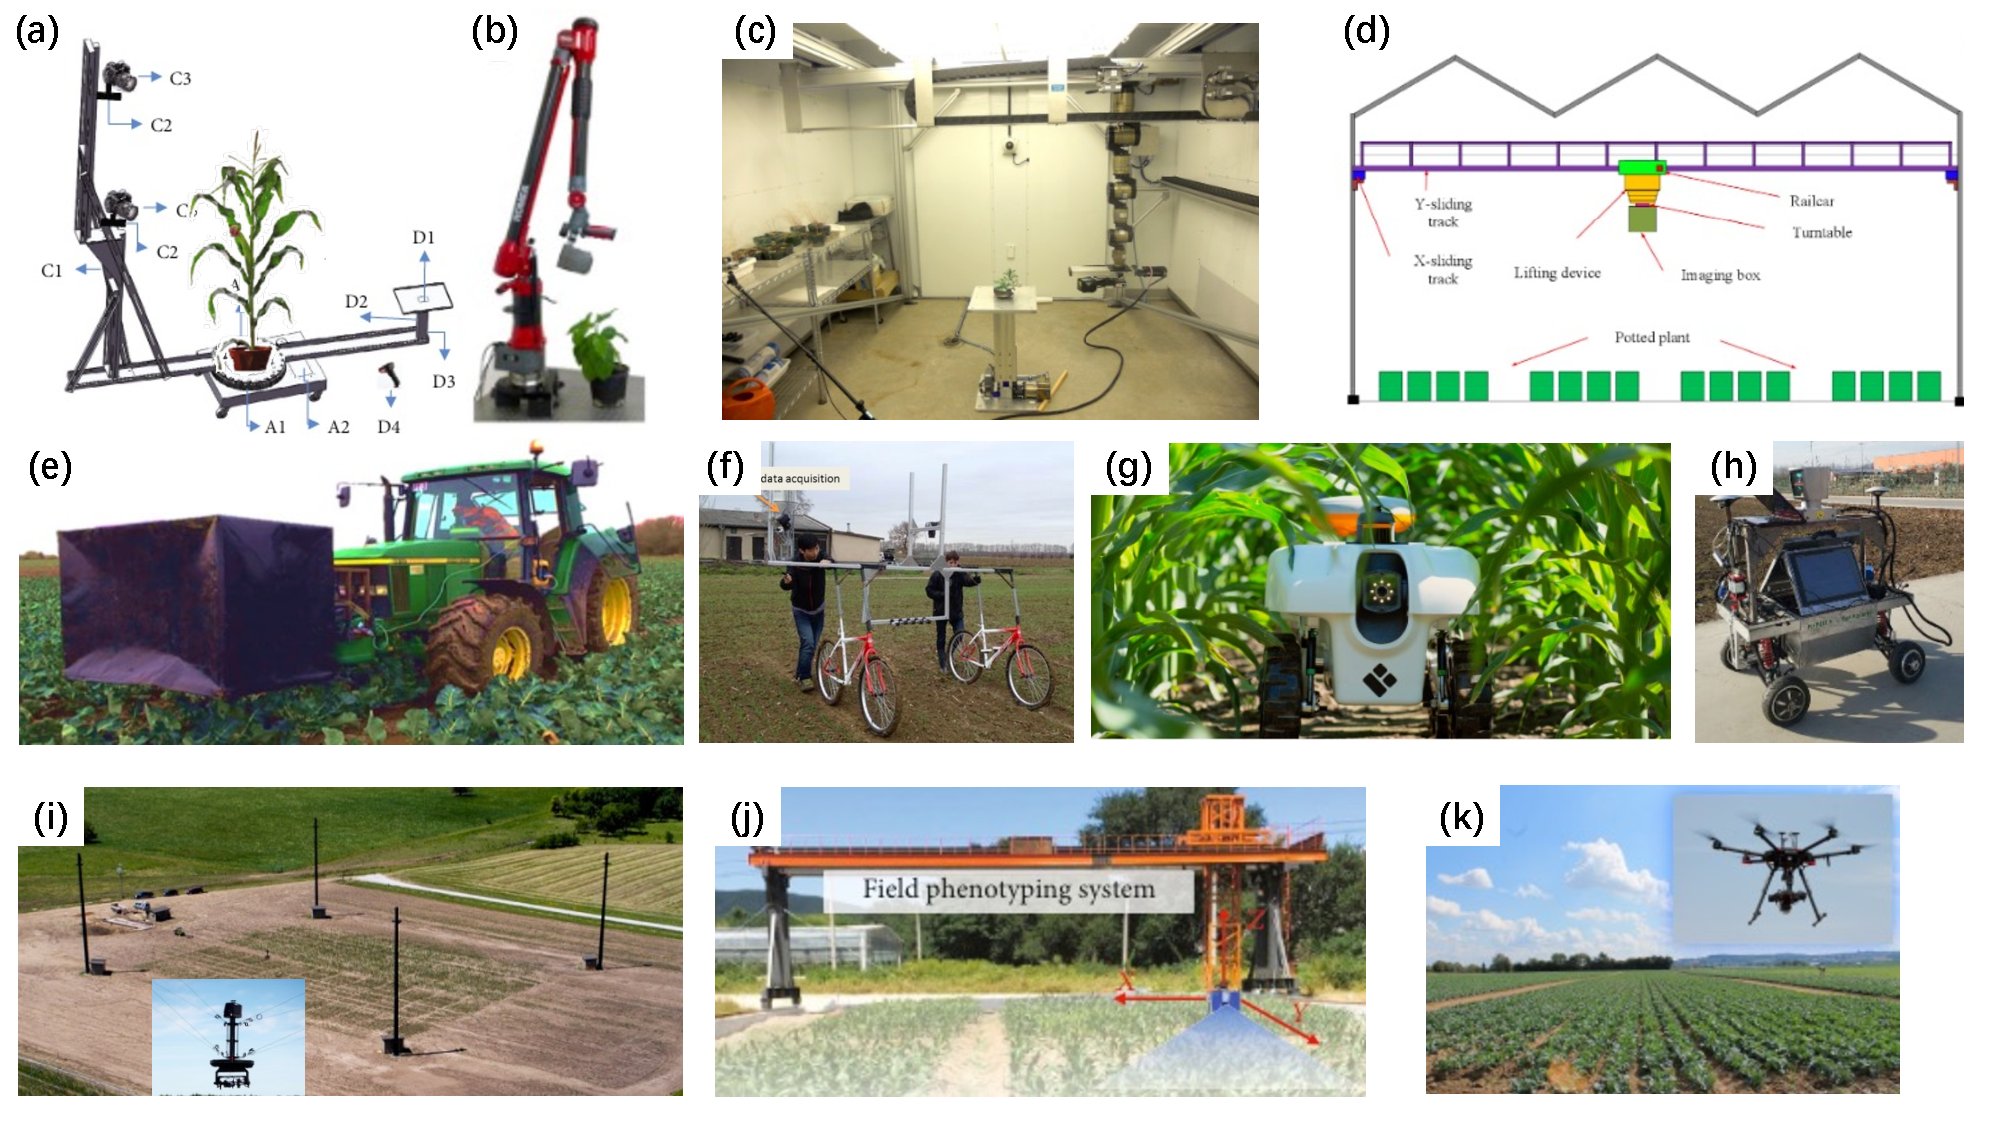
\includegraphics{figures/int/platforms.pdf}
    }
  \end{center}
  \caption[Example of platforms for plant phenotyping]{
    Example of platforms for plant phenotyping. (a-b) self-designed indoor devices \citep{wu_mvs-pheno_2020,schunck_pheno4d_2021}; (c-d) robotic arms in growth chamber or greenhouse \citep{chaudhury_machine_2018, du_greenhouse_2021}; (e) tractor \citep{kusumam_3d_2017}; (f) ground vehicle \citep{liu_estimation_2017}; (g-h) \gls{ugv} \citep{mcguire_high_2021, qiu_field-based_2019}; (i-j) robotic outdoor instruments \citep{bai_nu-spidercam_2019, jin_exploring_2021}; and (k) \gls{uav} \citep{kierdorf_growliflower_2022}
  }
  \label{fig:int1}
\end{figure}

% From the indoor to the outdoor, the commonly used platforms include self-designed indoor devices \citep{wu_mvs-pheno_2020,schunck_pheno4d_2021}, robotic arms in growth chamber or greenhouse \citep{chaudhury_machine_2018, du_greenhouse_2021}, tractor \citep{kusumam_3d_2017,blok_effect_2021}, ground vehicle \citep{liu_estimation_2017}, \gls{ugv} \citep{mcguire_high_2021,qiu_field-based_2019}, robotic outdoor instruments \citep{bai_nu-spidercam_2019, jin_exploring_2021}, \gls{uav} \citep{kierdorf_growliflower_2022, jang_review_2020}, and even satellite \citep{nguyen_monitoring_2020}. The scale of collected data using these platforms also changes from organ level, individual level to canopy level.

An important part of plant sensors is imaging sensors, which can record the morphological information of crops and are therefore commonly used in many plant phenotyping studies \citep{paulus_measuring_2019, feng_comprehensive_2021}. For example, the infrared, multi- and hyper-spectral imaging sensors were used to calculate several vegetation indices \citep{han_modeling_2019}, like \gls{ndvi}, to assess biomass \citep{jimenez-berni_high_2018}, yield and water stress level \citep{herrero_yield_2020, romano_use_2011}, and broccoli head freshness \citep{guo_evaluation_2022}. The common \gls{rgb} camera was also used to count plant number \citep{liu_estimating_2022}, plant density \citep{velumani_estimates_2021}, detect the broccoli head \citep{blok_machine_2016}, and access broccoli head quality \citep{stansell_use_2017}. They show the feasibility of imaging sensors in plant phenotyping with great efficiency and non-destructive dependency.

%% 3D sensors
% introduction for 3D phenotyping, method to obtain 3D (passive, active) -> cost limit, choose RGB+SfM
However, these imaging sensors are hard to directly describe the 3D morphological structure of plants, due to occlusion and dimension loss when projecting onto the 2D plane of photosensitive elements. As a result, it produces inaccuracies and uncertainties in 3D structure descriptions. With the development of sensing techniques, several studies reviewed the latest available approaches for 3D plant phenotyping \citep{paulus_measuring_2019, okura_3d_2022, kochi_introduction_2021}. Figure~\ref{fig:int2} summarizes some of them which are consisted of active and passive scanners. \citet[Table 5]{bartol_review_2021} also provide a complete list of commercial 3D scanners.

\begin{figure}[htb!]
  \begin{center}
    \resizebox{\textwidth}{!}{
      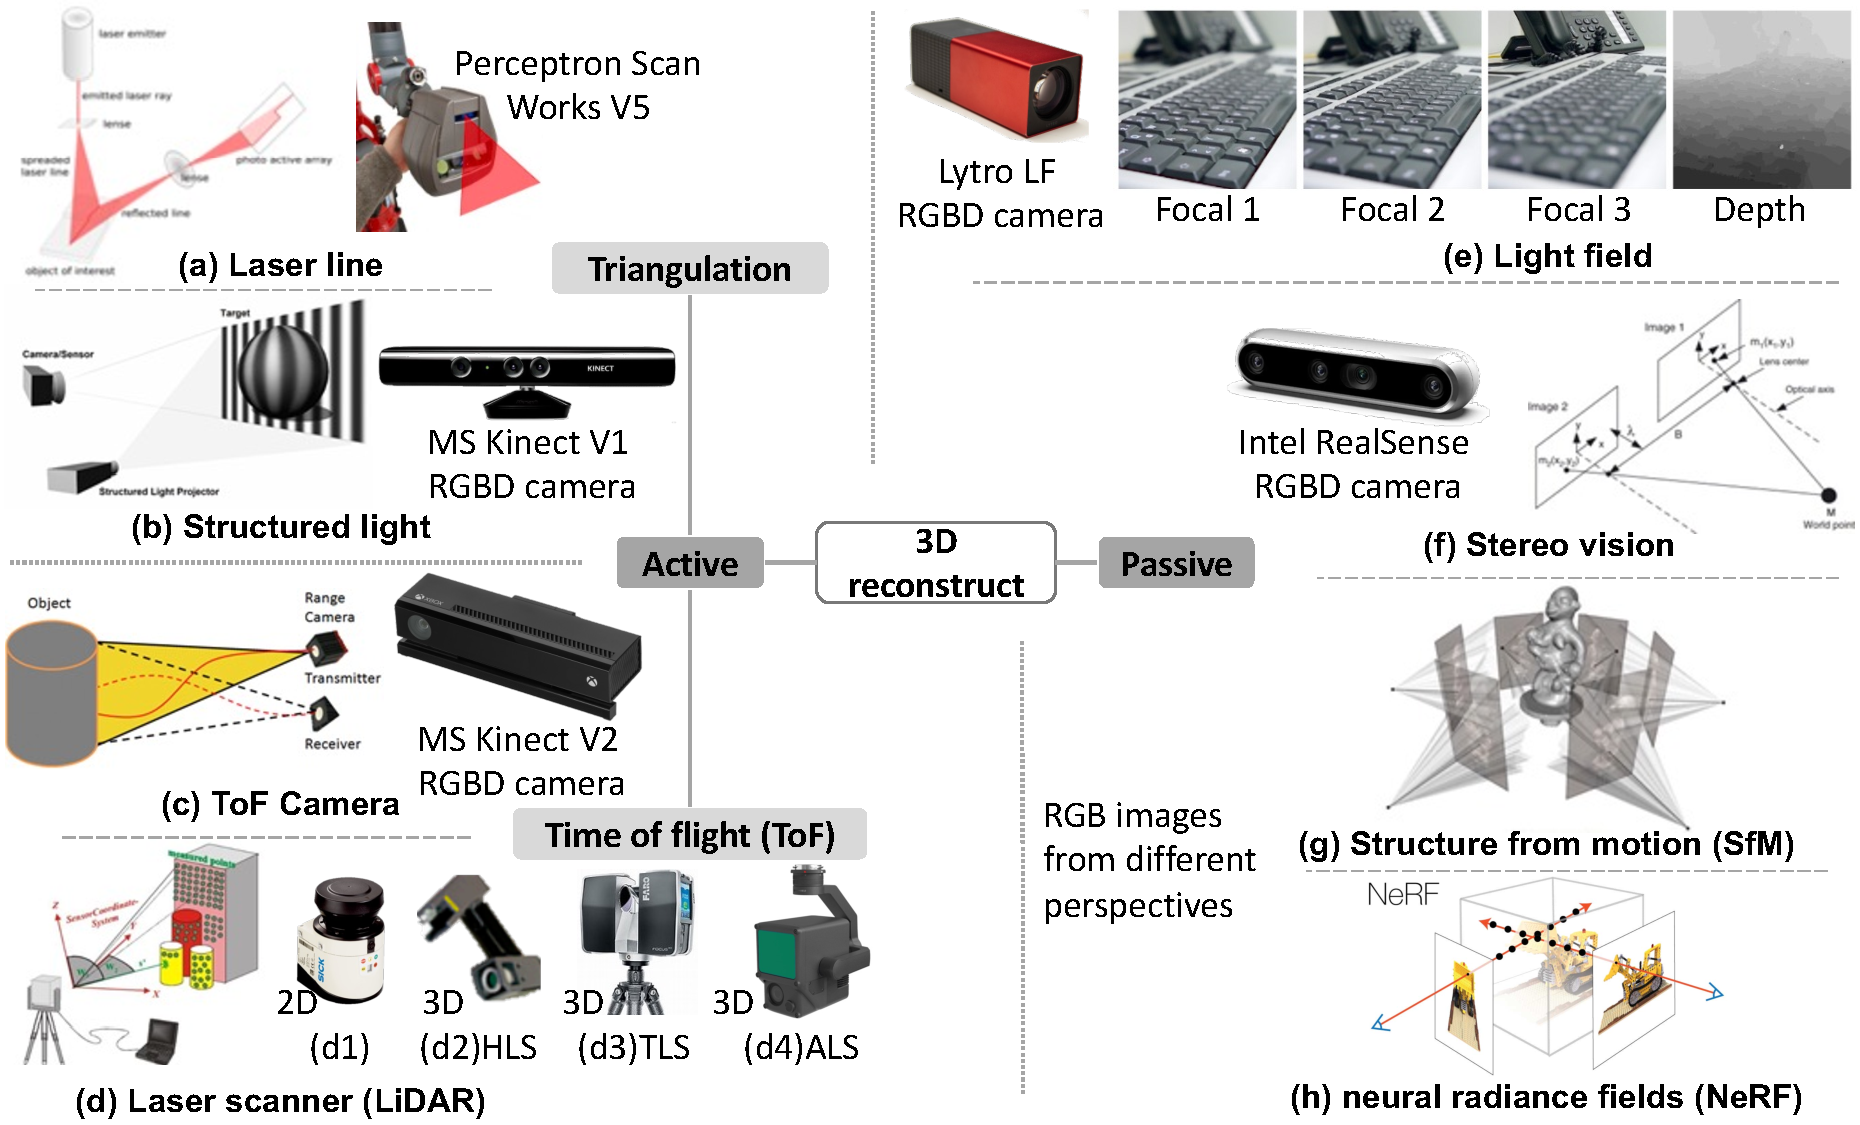
\includegraphics{figures/int/recons_sensors.pdf}
    }
  \end{center}
  \caption[Common methods for 3D structure reconstruction]{
    Common methods for 3D structure reconstruction. (a-d) The active sensors rely on projecting lights on the object and analyzing the reflection results, where (d) \acrfull{lidar}; (d2) \acrfull{hls}; (d3) \acrfull{tls}; (d4) \acrfull{als}; (e-g) the passive sensors rely on analyzing the passively received image groups. 
  }
  \label{fig:int2}
\end{figure}

The active scanners use a light source projecting on the object and analyze the reflection results to obtain the structure. It has two main parts, triangulation and \gls{tof}. The triangulation approach uses the shape changes on the projected straight laser line(s) to obtain the object structure. For example, \citet[Figure~3]{schunck_pheno4d_2021} used a laser line (Fig.~\ref{fig:int2}a) triangulation scanner (Perceptron Scan Works V5, Perceptron Inc., USA) to build a public 3D model database for maize and tomato. The structured light improved the efficiency by projecting an array of lines, often visible or infrared light rather than laser (Fig.~\ref{fig:int2}b). The Microsoft Kinect V1 is a famous \gls{rgbd} camera based on this approach which was released in November 2010. But it was used by a few plant phenotyping studies \citep{nguyen_structured_2015}, since the second version (Kinect V2, released in July 2014) and the third version (Azure Kinect, released in March 2020) with a different \gls{tof} approach and better performance \citep{tolgyessy_evaluation_2021, lachat_assessment_2015} were available. The \acrfull{tof} measures the distance between the sensor and points on the object to obtain its structure. According to the type of light source used, it can be divided into two categories: infrared for \gls{tof} camera (Fig.~\ref{fig:int2}c) and laser for \gls{lidar} (Fig.~\ref{fig:int2}d). Since the sun is a massive source of infrared, infrared-based ToF cameras typically do not perform well in outdoor environments with intense sunlight \citep{tolgyessy_evaluation_2021}; and are therefore commonly used for indoor plant reconstruction applications \citep{martinez_low_2019, zhang_3d_2020, xu_global_2023}. In contrast, the laser is often more tolerant to sunlight due to its stronger energy density, making it widely used in outdoor environments. According to the type of \gls{lidar} sensor, the 3D plant phenotyping applications are consisted of 2D \gls{lidar} scanner \citep{garrido_3d_2015}, 3D \gls{hls} \citep{ma_calculation_2019}, 3D \gls{tls} \citep{wu_accurate_2019, su_estimation_2018, qiu_field-based_2019}, and 3D \gls{als} \citep{ten_biomass_2019, nguyen_uav_2023}.

The passive scanners rely on analyzing the passively received image groups, mainly using the \gls{rgb} images. The light field camera takes a group of photos with different focal lengths, and the object structure is calculated according to different degrees of clarity caused by the different distances to the sensor (Fig.~\ref{fig:int2}e). For example, \citet{apelt_phytotyping_2015} built a light field camera system for measuring the morphological traits that are related to plant growth. A commercial low-cost light field camera (Lytro LF, Lytro Inc., USA) was used as \gls{rgbd} camera to monitor maize 3D morphological traits \citep{schima_imagine_2016}. While another commercial \gls{rgbd} camera, Intel RealSense (Intel Corporation, USA) uses a stereo vision approach (Fig.~\ref{fig:int2}f). It uses binocular vision like human eyes to obtain the object's structure. \citet{blok_image_2021} used this RealSense \gls{rgbd} camera to estimate the broccoli head size with different degrees of occlusion, which is a tough problem for common \gls{rgb} cameras. The photogrammetry approach is based on \gls{rgb} images obtained from different perspectives (view angles) using common imaging sensors (Fig.~\ref{fig:int2}g). It first uses the overlapped area among images to estimate the camera poses and object rough 3D structure (tie points), called \acrfull{sfm}. Then the \gls{mvs} is applied to densify the 3D point cloud of the tie points, and surface reconstruction and texture rendering are applied to obtain 3D mesh model of objects. For more details, please refer to \citep{hartley_multiple_2000,snavely_scene_2010}. 

% The structure from motion
%% software SfM
% ground sfm {Wu_MVS-Pheno_2020, Wang_Maize_2019, zhu_quantification_2020}; aerial sfm: {Liu_field-based_2021}
Unlike the previously mentioned scanners (Fig.~\ref{fig:int2}a-f) which often require a special not so ``low-cost'' devices, the \gls{sfm} approach only requires the \gls{rgb} camera and \gls{sfm} software with very flexible cost advantages. For the camera/sensor parts, even cameras of smartphones at hand can be used to obtain photos for plant modeling \citep{li_measuring_2020}. If require obtaining 3D plant models with ultra-high quality, the \gls{dslr} camera (over 4K resolution) can also be used to rise the 3D model quality to a higher level \citep{nguyen_3d_2016, drofova_use_2023}, which often exceeds the resolution of previously commercial \gls{rgbd} camera (around 1080p resolution). Meanwhile, a large amount of \gls{sfm} open-source and commercial software are available for individual plants (close-range) and geo-referenced canopy (aerial) purposes (Table~\ref{tbl:int1}). Due to this reason, many studies applied it for obtaining the 3D models of indoor individual plants \citep{wu_mvs-pheno_2020, zhou_automated_2019}, in-field individual plants \citep{jay_field_2015, herrero_structural_2023}, and in-field canopy \citep{kim_modeling_2018, herrero_canopy_2020}.

\begin{table}[htb]
  \caption[Softwares for 3D reconstruction using photogrammetry]{Softwares for 3D reconstruction using photogrammetry; ``Close-range'' is mainly used for building 3D models of individual plants or organs at the local coordinate; ``Aerial'' is mainly used for building geo-referenced canopy 3D models using \gls{uav} imagery with \gls{gps} coordinates.}
  \label{tbl:int1}
  % \begin{adjustwidth}{-0.05\textwidth}{-0.05\textwidth}
    \begin{center}
    % \resizebox{0.9\textwidth}{!}{
      \begin{threeparttable}
      \begin{tabular*}{\linewidth}{@{\extracolsep{\fill}} clcc}
        \hline
        \multicolumn{1}{c}{\textbf{Types}} & \multicolumn{1}{c}{\textbf{Software name}}                                                                      & \textbf{close-range} & \textbf{aerial}     \\ \hline
        Open source                        & AliceVision Meshrooms                                                                                           & $\checkmark$         & $\checkmark$        \\
                                           & COLMAP                                                                                                          & $\checkmark$         & $\checkmark$        \\
                                           & Multi-View Environment (MVE)                                                                                    & $\checkmark$         & $\times$            \\
                                           & OpenDroneMap\tnote{1}                                                                                           & $\times$             & $\checkmark$        \\
                                           & OpenMVG $\stackrel{2}{\rightarrow} \begin{cases} \text{MVE} \\ \text{OpenMVS} \end{cases}$                      & $\checkmark$         & $\checkmark$        \\
                                           & VisualSFM $\stackrel{2}{\rightarrow} \begin{cases}\text{MeshRecon}\\ \text{OpenMVS} \\ \text{PMVS} \end{cases}$ & $\checkmark$         & $\bigcirc$\tnote{3} \\
        Commercial                         & 3DF Zephyr                                                                                                      & $\checkmark$         & $\checkmark$        \\
                                           & Agisoft Metashape                                                                                               & $\checkmark$         & $\checkmark$        \\
                                           & Autodesk Recap Photo                                                                                            & $\checkmark$         & $\checkmark$        \\ 
                                           & ContextCapture                                                                                                  & $\checkmark$         & $\checkmark$        \\
                                           & Correlator3D                                                                                                    & $\times$             & $\checkmark$        \\
                                           & DJI Terra \tnote{4}                                                                                             & $\times$             & $\checkmark$        \\
                                           & DroneDeploy                                                                                                     & $\times$             & $\checkmark$        \\
                                           & Elcocision 10                                                                                                   & $\checkmark$         & $\checkmark$        \\
                                           & Pix4Dmapper                                                                                                     & $\times$             & $\checkmark$        \\
                                           & Reality Capture                                                                                                 & $\checkmark$         & $\checkmark$        \\ \hline
      \end{tabular*}
      \begin{tablenotes}
        \footnotesize
        \item[1] charges for a complied installer for whom is difficult to install from source code;
        \item[2] some software only provide \gls{sfm} pipeline, need to integrate them with \gls{mvs} software as a complete 3D reconstruction pipeline;
        \item[3] has video tutorials for processing UAV images, but no official documentation about making geo-referenced GeoTiff for common aerial products like \gls{dom} and \gls{dsm};
        \item[4] is optimized for DJI (Shenzhen DJI Technology Co., Ltd. China) drones only.
      \end{tablenotes}
      \end{threeparttable}
    % }
    \end{center}
  % \end{adjustwidth}
\end{table}

Recently, for the \gls{cg} industry which often needs to scan objects to 3D models and render images from different perspectives, \citet{mildenhall_nerf_2022} proposed a novel deep learning method (Fig.~\ref{fig:int2}h). The proposed \gls{nerf} approach is just based on the \gls{sfm} step and can skip the time-consuming \gls{mvs}, 3d meshing and 3D rendering steps of photogrammetry. It showed the feasibility of obtaining plant 3D structures from the official demo (\url{https://www.matthewtancik.com/nerf}) and \citet{jignasu_plant_2023} obtained the maize 3D structure using this approach. But this approach heavily relies on the training data; there are plenty of datasets available for industrial applications, and for agricultural applications at the current stage, the manual collecting training data using \gls{lidar} is required \citep{jignasu_plant_2023}. Its application in agriculture has not shown significant advances over the mature photogrammetry approach and still needs further development at the current stage.

% Considering the maturity of technology and the cost of sensors, the low-cost and mature photogrammetry approach (Fig.~\ref{fig:int2}g) has been chosen to collect research data in this study.

% \subsection{Data analysis for phenotyping}
% for data analysis.

\subsection{ROI extraction}

After collecting the data, the following step is extracting the \acrfull{roi} for further analysis. The \gls{roi} can have different meanings for different research purposes. For canopy-level studies or breeding studies, the \gls{roi} is the regions within each plot boundary \citep{trevisan_htp_2020, han_drone_2021}; For individual-level studies, the \gls{roi} is the plant parts without involving any background like soils or weeds \citep{ge_method_2019,guo_fieldbased_2020}; For organ-level studies, the \gls{roi} is the part of each organ without the other parts of the plant, for example, the broccoli head \citep{zhou_monitoring_2020} and sorghum tassel \citep{ghosal_weakly_2019} without leaves. In this section, different image analysis and 3D data analysis methods and algorithms are summarized for the 2D image collected from imaging sensors and 3D models (e.g. 3D point cloud) from 3D photogrammetry or \gls{lidar} scanner, respectively.

\subsubsection{Full field data preprocessing}

% plot region extraction (canopy level)
% easympe, other plot segments
For canopy-level or full-field phenotyping applications, the \gls{dom} is often used as the field plot map (by \gls{uav} photogrammetry); the 3D point cloud is often used as 3D canopy models (by photogrammetry or \gls{lidar} scanner). However, processing the whole file image or 3D data directly is often impossible, since the file size of these whole canopy data is very large (often over 0.5GB and can reach 10GB+). One common data preprocessing of plant phenotyping applications is splitting the whole field into smaller parts \citep{wang_easyidp_2021}. It can be split by either equal-size grids (e.g. \citet{bauer_combining_2019} split full \gls{dom} image to several 250$\times$250 pixel grids) or the boundary of each (micro)plot \citep{tresch_easympe_2019}, the latter one is more meaningful and often used.

To place plot boundaries and their labels on the \gls{dom} map manually, the \gls{gis} software like ArcGIS Desktop (Esri, Redlands, USA) and QGIS (open source, \url{https://qgis.org}) are often used. The (micro)plot results are often saved in shapefile format (*.shp) for better compatibility with other software. However, manually editing and operating software \gls{gui} is time-consuming for large fields, hence several studies tried to solve the automatic \gls{roi} detection and generation by computer vision. \citep{tresch_easympe_2019} developed an open-source python package EasyMPE to generate and crop \gls{roi} semi-automatically. This tool was then later re-built using C++ by \gls{naro}, named PREPs (\url{http://cse.naro.affrc.go.jp/aitoh/PREPs}), for higher performance on the Windows platform. \citet{chen_grid_2020} also developed a similar tool using python name GRID (\url{https://zzlab.net/GRID}); \citet{mortensen_drone_2019} developed the using the Matlab; and \citep{sara_automatic_2021} extended them by supporting slightly adjusting the \gls{roi} location to fit better with the canopy. All these tools also support cropping the full \gls{dom} to small parts within the \gls{roi} for postprocessing.

For the 3D canopy point cloud, the point cloud processing software like MeshLab (open source, \url{https://www.meshlab.net}) or CloudCompare (open source, \url{https://www.cloudcompare.org}) are often used for similar \gls{roi} cropping tasks but not very convenient. Instead, it is more often to use the \gls{roi} shapefiles made in the previous step and write batch scripts for processing. For example, \citet{sun_field_2018} cropped the \gls{roi} on \gls{lidar} point cloud using the Matlab script but not they did not publish their code. Thus, we developed the EasyIDP python package for processing the \gls{dom} and point cloud more easily \citep{wang_easyidp_2021}. After preprocessing the full field into smaller parts, the following ``2D image analysis'' and ``3D data analysis'' can be applied for each part.

\subsubsection{2D-based approaches}

Most of the image analysis tasks for plant phenotyping can be summarized into three categories: classification, detection and segmentation. The classification task is to determine what class of objects are in a given image. For example, decide whether a broccoli head image is healthy or diseased \citep{garcia_towards_2021}. The detection task combines classification and localization, it can tell what kind of object and where are they in the given image. For example, detect how many maize buds \citep{liu_estimating_2022} or sorghum tassel \citep{ghosal_weakly_2019} and their locations in the image. The segmentation task separates a given image into several regions with particular shapes and borders. It consists of semantic segmentation and instance segmentation. Semantic segmentation shares the same label with all the objects that belong to the same class (e.g. where is the region of plants or broccoli heads in an image), while instance segmentation produces unique labels for each object (where are the regions of each broccoli head in an image). These tasks are not isolated from each other. For example, for semantic segmentation, the conventional computer vision method is to classify each pixel to obtain the segmentation result of the entire image \citep{guo_easypcc_2017}; while instance segmentation usually requires the combination of the results of semantic segmentation and detection to achieve the identification of each individual's region \citep[Fig.~2]{luling_using_2021}.

% [todo] a figure about broccoli detection, sematic segmentation, and instance segmentation.

%%% traditional CV method
The most conventional attempts are trying to use computer vision algorithms on common \gls{rgb} images. In some simple cases, a manually defined color threshold can be used for separating plants from backgrounds. For example, \citet{choudhury_holistic_2018} converted the maize plant image from \gls{rgb} to \gls{hsv} and used ``\textit{hue (range 0.051-0.503), saturation (range: 0.102-0.804) and value (range 0.000-0.786)}'' to separating plant regions from the background. However, in most outdoor images with complex lighting and background conditions, the manual thresholding does not have good performance. Thus, \citet{meyer_verification_2008} proposed the color vegetation indices (NDI, ExG and ExR) and combined with \citet{otsu_threshold_1979} thresholding algorithms for automated crop imaging application. For better compatibility with more complex scenarios without being limited to green plants, \citet{guo_easypcc_2017} manually annotated the training data to train machine learning classifiers based on extended color information. Further, \citet{zou_broccoli_2019} and \citet{blok_machine_2016} segmented the broccoli buds and heads, respectively, using the texture and color information with the trained support vector machine (SVM) classifier.

%%% deep learning based method
%% -> 深度学习2D图像检测算法 siyuan
In the same way, deep learning techniques show great potential for better RGB image processing results. The \gls{cnn} is a famous deep learning framework for color imagery used by many phenotyping studies. \citet{ghosal_weakly_2019} used a pre-trained \gls{cnn} model for sorghum head detection and counting; \citet{liu_estimating_2022} applied the Fast \gls{rcnn} for counting the maize seedling number; \citet{bender_high_2020} applied the FastRCNN for detecting and segmenting the entire broccoli on the RGB images and shared them as public datasets; \citet{blok_effect_2021} simplified the MaskRCNN with data augmentation for broccoli head segmentation on RGB images. However, its accuracy is affected by the leaf occlusion; \citet{blok_image_2021} fixed this issue by using the \gls{orcnn} to recover the hidden head area; and \citet{garcia_towards_2021} also applied the FasterRCNN for distinguishing the immature and diseased broccoli. 
 
% convetional cv solution, but algriculutre also has many alternatives. (depth info, time-series info, hyperspectal)

\subsubsection{3D-based approaches}

Although 2D-based machine learning and deep learning approaches show the feasibility of extracting \gls{roi}s, for very complex scenes it often requires labeling a considerable number of training sets to ensure a better performance. The 3D-based approaches can not only provide more morphological information but also can greatly simplify complex tasks.

The depth information is often used as a common and simple 3D-based approach. The depth image is a common file format for that information, which uses pixels to record depth values. It can be obtained from either depth cameras (often for close-range, the depth value is the distance from the object to the camera) or photogrammetry (often for aerial, the depth value is the height or altitude). Such information has been widely used for better plant segmentation for phenotyping studies. For close-range applications, \citep{luling_using_2021} used the depth image generated by photogrammetry and the color information to segment cabbage instances. For the aerial photogrammetry applications, \citet{guo_fieldbased_2020} segmented the plant area inside each \gls{roi} using the color and the depth information from \gls{dom} and \gls{dsm} respectively. 

Another format for recording the depth information is the 3D point cloud, and the 3D point cloud analysis is also of great importance for the 3D-based approach. Before processing, due to the disorderliness of the data structure of the point cloud, point downsampling and noise removal are required to decrease the data size and processing difficulties \citep{ma_calculation_2019}. 

Then, a semantic segmentation between plants and background (e.g., soil) is required. Color thresholding mentioned in the 2D-based approach also works for 3D point clouds with colors. \citet[Fig.~3]{xiao_image-based_2020} manually defined \gls{rgb} threshold ($R-G\geq7$) for separating plant points from backgrounds like shadow and soil points. The geometry relationship among points can also be used for segmentation. \citet{ge_method_2019} applied the \gls{gmm} clustering to recognize the points of broccoli buds and remove the discrete points (noises) by \gls{knn} algorithm. While instead of extracting plant parts, \citet{garrido_3d_2015} used the \gls{ransac} plane regression to find out the flat ground points and removed them.

After semantic segmenting the plant part, the instance segmentation to split each plant should proceed for the individual-level studies. \citet{hofle_radiometric_2014} developed a region-growth method based on the local maxima in elevation to split each maize bud from semantic segmented points. It shared a similar idea of \gls{dbscan} clustering method which is used by several studies later for maize \citep{lin_segmentation_2022} and cotton balls \citep{sun_3d_2020}. \citet{kusumam_3d_2017} detected two broccoli varieties' heads by Euclidean clustering method and the SVM classifier on the 3D features and \citet{montes_real-time_2020} further expanded it to almost real-time detection for the actual applications.

Finally, the organ-level studies require segmentation on each organ, especially for crops with complex morphological structures (e.g. maize, tomato). According to morphological characters of different crops or cultivars, different studies proposed different solutions. For the tasks of maize leaf segmentation, \citet{jin_stemleaf_2019} proposed a \gls{mnvg} algorithm; \citet{liu_canopy_2021} used skeletonize and region growth; \citet{wang_dfsp_2023} proposed a distance field-based segmentation pipeline; and \citet{miao_label3dmaize_2021} used the optimal transportation distance and published an interactive segmentation tool (Label3Dmaize, \url{https://github.com/syau-miao/Label3DMaize}). For the tomato stem and leaf segmentation, \citet{rossi_implementation_2022} proposed a complex but automatic workflow using the Matlab, including radius detection, sphere climbing, and phyllotaxy retrieving. \citet{helin_using_2023} proposed a t-distributed stochastic neighbor embedding segmentation method and proved its feasibility on five different plants (hibiscus, maple, tomato, tobacco and rosebush). \citet{dutagaci_rose-x_2020} and \citet{schunck_pheno4d_2021} even published an annotated dataset for evaluating 3D plant organ segmentation methods.



%  or deep learning method \citep{jin_deep_2018}.


%% 棉花点云

%% 3D data analysis

%%% remove background

% combine with depth info



%%%% individual segmentation

%%%% organ segmentation

%%% how to do 3D deep learning: (思源笔记,三维深度学习的种类)

\subsection{Traits calculation and applications}
% du_greenhouse_2021 -> 100多个参数

%% 1D 参数

%% 2D 参数
% Hundreds of static and dynamic traits related to geometry, structure, texture, and colors on lettuce were measured by a self-designed high-throughput phenotyping platform [2\citep{du_greenhouse_2021}]. 

%% 3D 参数
% After segmenting point cloud to part of interest, the simple traits such as maize height [4,13]\citep{hammerle_mobile_2018,qiu_field-based_2019}, row spacing \citep{qiu_field-based_2019}, plant skeleton \citep{wu_accurate_2019} and biomass \citep{jin_non-destructive_2020} could be calculated, and also some advanced application for drought stress \citep{su_evaluating_2019}, intercropping \citep{liu_field-based_2021} and light competition \citep{zhu_quantification_2020} analysis.

% skeleton extraction.



% \subsection{Advanced applications}

%% 时间序列分析的文献(使用时间序列追踪参数的变化) 思源笔记
% they were used for discovering the loci regulating flower opening [11\citep{han_drone_2021}].

%% 收期预测、光照模拟, 辅助QTL

% The lettuce growth and photosynthetic performance reaction to drought stress were also assessed [\citet{sorrentino_lettuce_2020}]. 

\section{Challenges in plant phenotyping}

%% 上述的三维分析方法,仅限于高质量的点云?对于大部分来说,质量不够很难进行3D的分析

%% 数据集标注的工作量问题
Besides, the model selection and parameter adjustment of machine learning as well as the training data preparation of machine learning, are still highly dependent on expert experiences and intensive labor. The auto machine learning framework and weakly supervised learning have merged as the interesting candidate to solve such dilemma.

\section{Objective of this study}

\begin{enumerate}
    \item To develop an almost-automatic 3D reconstruction workflow that can obtain the integrate and high-quality 3D models of destructively sampled broccoli heads.
    \item To develop an unsupervised phenotyping workflow that can automatically segment the broccoli crown part from Objective 1, and calculate several 1D to 3D morphological traits.
    \item To develop an improved workflow for \gls{uav}-based 3D reconstruction broccoli canopy using the 3D to 2D projection and labor-saving deep learning technique, which can obtain better 2D morphological traits of broccoli heads in complex outdoor conditions.
    \item To combine the strengths of the \gls{uav}-based pipeline (high throughput but low quality) and the destructive-based pipeline (high quality but low throughput). Using the auto machine learning regression and the template matching to recover the 3D traits from \gls{uav}-based 2D traits for all broccolis in the field.

\end{enumerate}


\section{Outline of this study}

Chapter 1 is an overview of the study's background information, relative studies, and objectives

Chapter 2 develops and validates the 3D phenotyping pipeline for destructively sampled broccoli heads using the photogrammetry technique, which includes obtaining high-quality plant 3D models and calculating the 3D traits.


Chapter 3 develops and validates the 3D phenotyping pipeline for \gls{uav} sensing on broccoli canopy, includes the 3D to 2D projection pipeline to improve deep-learning-based phenotyping

Chapter 4 tests the idea of cross-scale assimilation of broccoli based on the pipeline built in Chapter 2 and Chapter 3.

Chapter 5 summarizes the general conclusions of this study, and also discusses the research prospects in the future.